\setchapterstyle{kao}
\setchapterpreamble[u]{\margintoc}
\chapter{Can Analysis} 
\labch{51CA}

\section{Function Description}
The ZLG CANOpen Analysis is used for the controlling of Rope-Climbing Robot climbing motor, it should be 
used with Can Analysis \ref{ch:34RMD}. 
% \sidenote{  \href{https://www.akm.com/cn/zh-cn/technology/technical-tutorial/basic-knowledge-magnetic-sensor/hall-sensors/}
% {Introduction of Hall sensors link} }. 
% \begin{figure}[hb]
% 	\includegraphics[width=0.45\textwidth]{4101_motor1.jpg}
% 	\caption[Mona Lisa, again]{It's Mona Lisa again.}
% 	\labfig{fig411_cleaningMotor}
% \end{figure}

Application: CANOpen protocol analysis.

\begin{figure}[htb]	
	\centering
	\begin{subfigure}
		\centering
		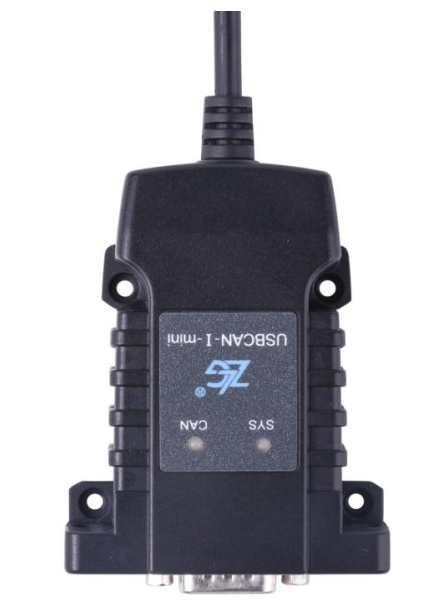
\includegraphics[width=2in]{5111_CA_I_mini.png}
		% \caption{motor with reduction detail}\label{fig:4101}		
	\end{subfigure}
	\quad
	\begin{subfigure}
		\centering
		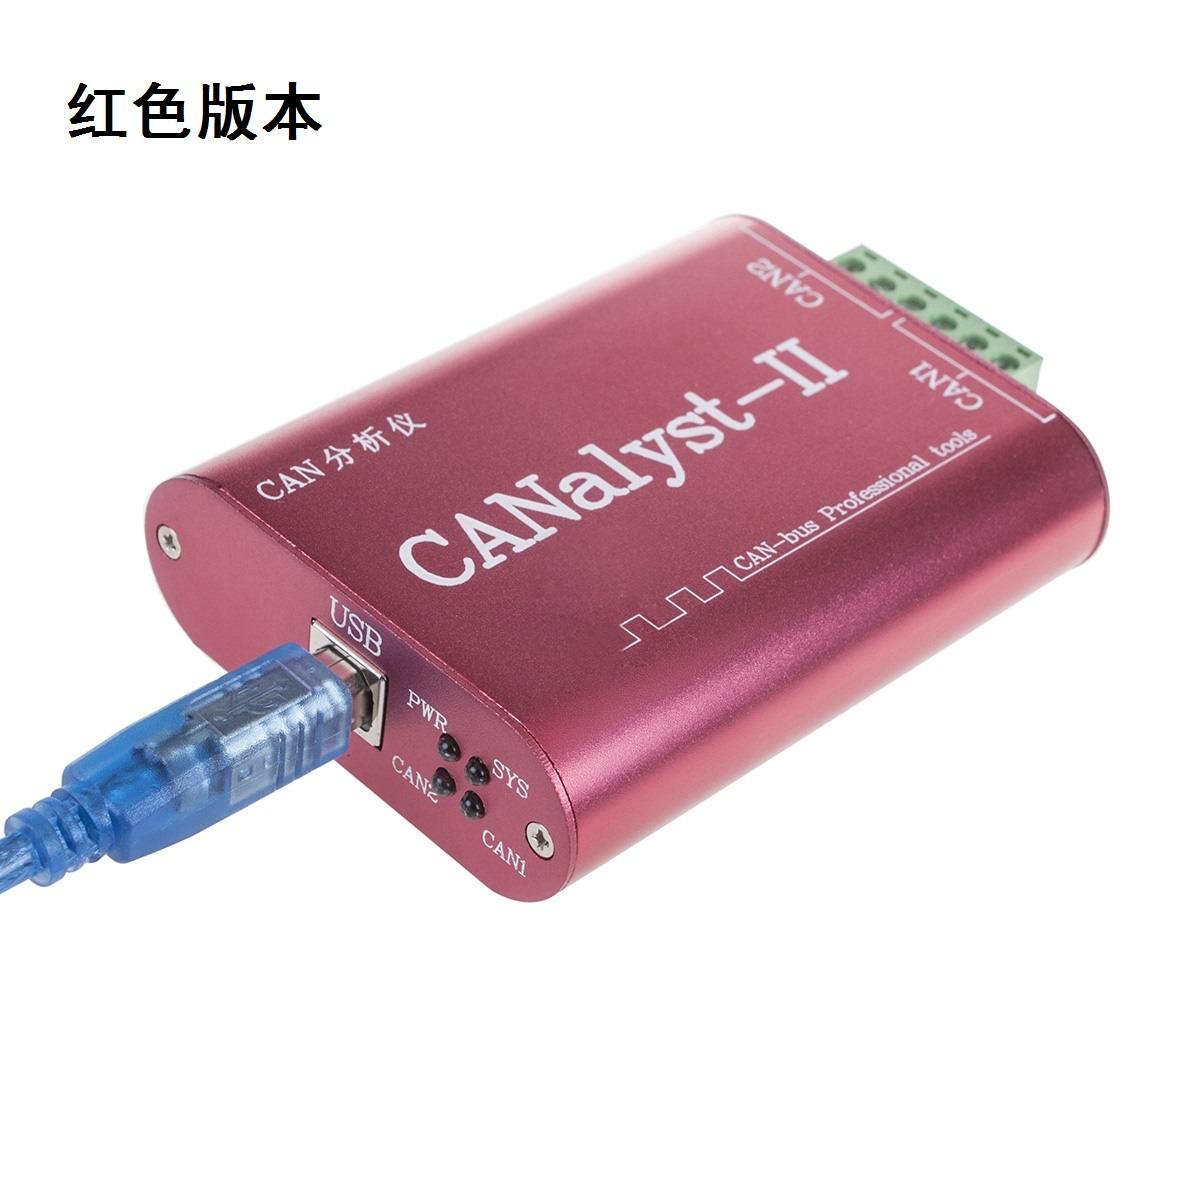
\includegraphics[width=2in]{5111_CA_II.jpg}
		% \caption{motor with brand}\label{fig:4102}
	\end{subfigure}
	% \begin{subfigure}
	% 	\centering
	% 	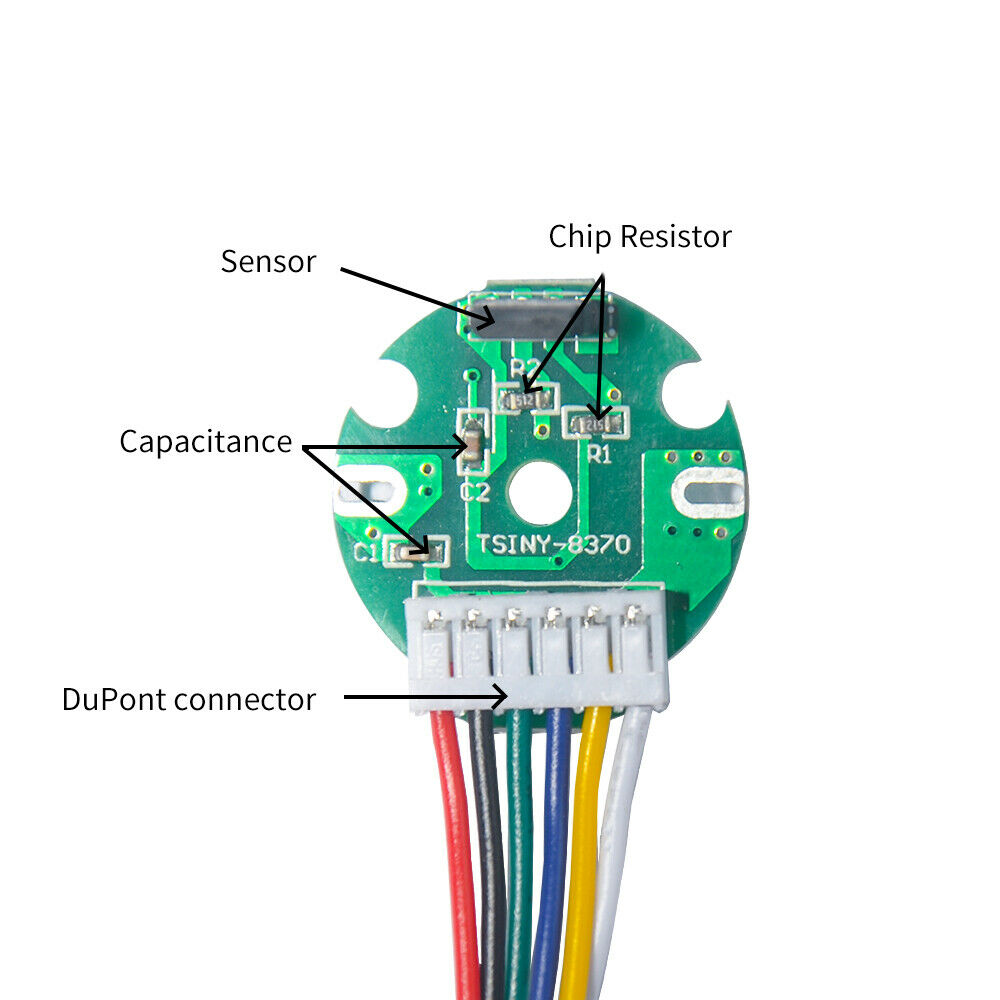
\includegraphics[width=2in]{412_hallencoder.jpg}
	% 	% \caption{motor with brand}\label{fig:4102}
	% \end{subfigure}
	\caption[ZLG CANOpen Analysis]{ 
		ZLG CANOpen Analysis	
			}\label{fig:510}
\end{figure}
% \marginnote[-12pt]{
	
% 	}
\section{Purchase Info}
Purchase:
\begin{enumerate}
	\item brand: ZLG(zhiyuan electrical)
	\item type: USBCAN-I-MINI
	\item link: \href{https://item.taobao.com/item.htm?id=582701516953&price=1199}{taobao link} 
	\item price: 1199RMB
	\item data: June. 2020
	\item RP: SGL, clear
\end{enumerate}

Supporting Material:
\begin{enumerate}
	\item ZLG download website: \url{https://www.zlg.cn/can/down/down/id/22.html}
    \item Always refer to: online instructions of USBCAN-I-MINI instruction, \url{https://manual.zlg.cn/web/#/63?page_id=2568} 
      They have been downloaded in ros package robomodule sheet folder on {\color{red} September 19, 2020.}.
	% \item telephone: +86-18503054370
    % \item rs232 serial wire purchase link: \url{https://detail.tmall.com/item.htm?id=39113690170 }
\end{enumerate}


\section{Instruction for Connection}

\begin{figure}[htb]
	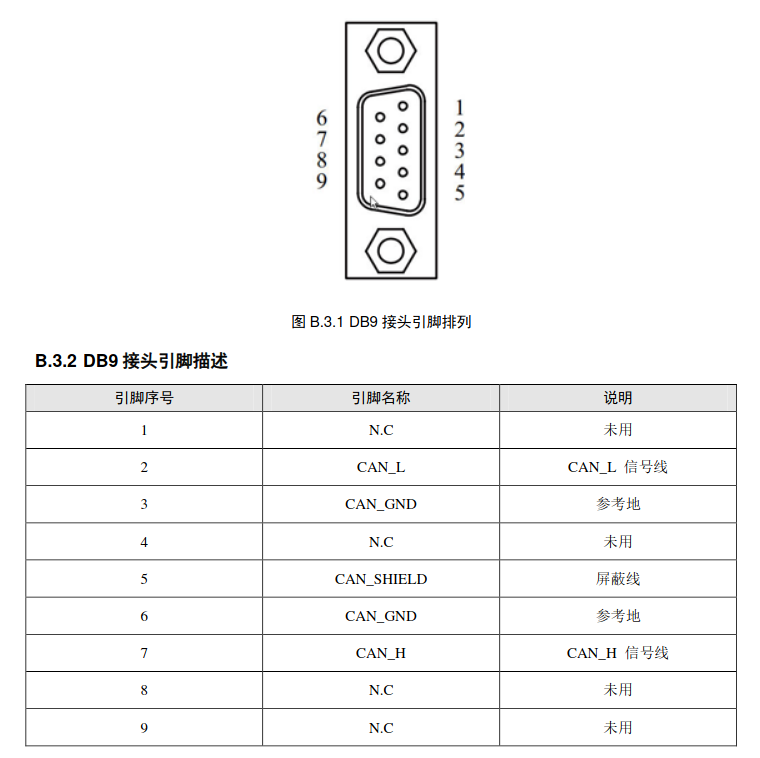
\includegraphics[width=1\textwidth]{5131_CA_DP9_canpin.png}
	\caption[Can Analysis DP9 pin]{ 
		Can Analysis DP9 pin.		 
		}
	\labfig{fig5131:CA}
\end{figure}
% 1234

% wire definition in encoders:
% \begin{enumerate}
% 	\item {\colorbox{red}W red}: M1, motor + positive
% 	\item {\colorbox{black}W black}: GND, encoder power supply - negative
% 	\item {\colorbox{yellow}W yellow}: C1, encoder signal A phase
% 	\item {\colorbox{green}W green}: C2, encoder signal B phase
% 	\item {\colorbox{blue}W blue}: 3.3/5v, encoder power supply + positive
% 	\item {\colorbox{white}W white}: M2, motor - negative 
% \end{enumerate}

\section{Mechanical Specification}

\begin{enumerate}
	\item USBCAN-I-mini:  W: 59mm, L: 75.5mm; H: 14mm
\end{enumerate}

% \begin{figure}[htb]
% 	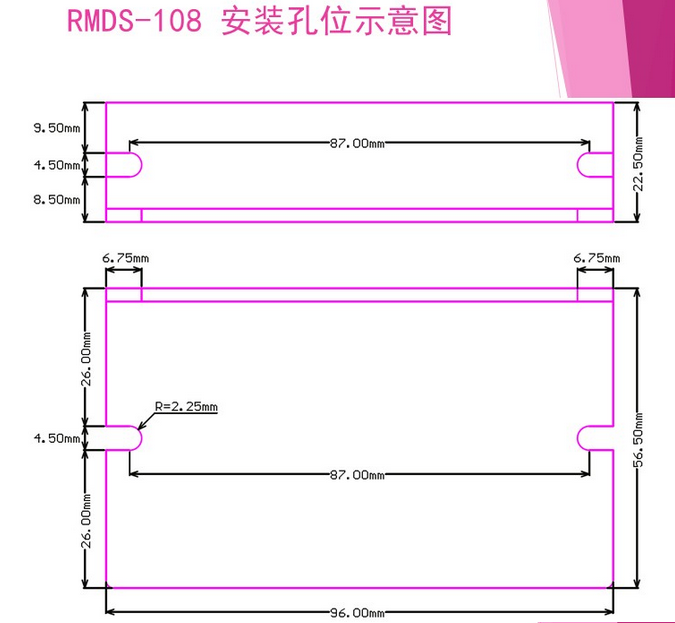
\includegraphics[width=0.8\textwidth]{3441_RMDS_109_mech_install.png}
% 	\caption[RMDS109 mechanical installation]{ 
% 		RMDS109 mechanical installation. (109 is same as 108), in 403,401, just care 87mm to 105mm		 
% 		}
% 	\labfig{fig3441_mech_install}
% \end{figure}

\section{Interface Library Notes}
\begin{description}
	\item[Device type] Different version of ZLG CAN has different device type, it should be set in the \textbf{demo\_config.yaml}.
	\item[Baudrate setup] Different CAN Baudrate should be set in the function: \textit{VCI\_INIT\_CONFIG}, in our file \textbf{can\_application.cpp}
% function: $\textit{VCI_INIT_CONFIG}$


\end{description}

\begin{table}[htb!]
	\caption[Device type number table]{Device type number table.}
	\labtab{511Candevicenumber}
	\begin{tabular}{ c c c }
		\toprule
		product type & library device name & device type number \\
		\midrule
		USBCAN-I/I+  & USBCAN1  &   3 \\
		\midrule
		USBCAN-II/II+ & USBCAN2 & 4 \\
		% \multirow{3}{4em}{Multiple row} & cell2 & cell3 & cell4\\ &
		% cell5 & cell6 & cell7 \\ &
		% cell8 & cell9 & cell10 \\
		% \multirow{3}{4em}{Multiple row} & cell2 & cell3 & cell4 \\ &
		% cell5 & cell6 & cell7 \\ &
		% cell8 & cell9 & cell10 \\
		\bottomrule
	\end{tabular}
\end{table}

\begin{table}[htb!]
	\caption[Can Analysis Baudrate timing set table]{Can Analysis Baudrate timing set table.}
	\labtab{512Baudrate}
	\begin{tabular}{ c c c }
		\toprule
		Can Baudrate & Timeing0 & Timing1 \\
		\midrule
		500Kbps  & 0x00  &   0x1C \\
		\midrule
		1000Kbps  & 0x00  &   0x14 \\
		\bottomrule
	\end{tabular}
\end{table}
% \section{others}
% \subsection{how to use 12v motor in 24v power supply }
% set in the windows GUI, set PWM and current limitation.
% \begin{figure}[!htb]
% 	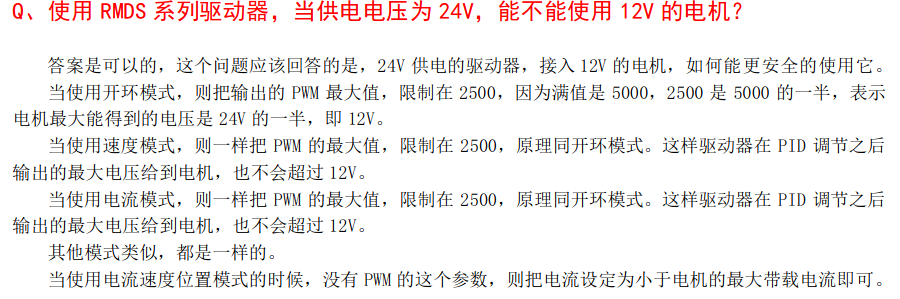
\includegraphics[width=0.8\textwidth]{345_use24vfor12vmotor.png}
% 	\caption[how to use 12v motor in 24v power supply]{ 
% 		how to use 12v motor in 24v power supply.		 
% 		}
% 	\labfig{fig:345}
% \end{figure}



